\chapter{Tema Secundário I : Programação Paralela}\label{tema3}


\section{Computação de Alto Desempenho}\label{Computação de alto desempenho}

O termo Computação de Alto Desempenho ou HPC (do inglês \textit{High-performance computing}) refere-se à prática de agregar o poder computacional de uma forma que proporciona um desempenho muito superior do que se poderia obter de um computador de mesa, a fim de resolver os grandes problemas da ciência, engenharia, ou de negócios. O uso eficiente desses recursos é o principal foco de estudo nessa área.

Em decorrência disso, criou-se a possibilidade de resolver problemas mais complexos como tratamento de conjuntos de imagens, biologia computacional, mineração de dados, simulação de modelos científicos e de engenharia entre outros.


\subsection{Classes de Arquiteturas Existentes}

Uma aplicação paralela pode ser composta por uma ou mais tarefas. As tarefas que compõem uma aplicação paralela podem executar em vários processadores, caracterizando desta forma o paralelismo da execução da aplicação. Os tipos de processadores utilizados por uma determinada aplicação e o meio de comunicação entre eles caracterizam a classe de arquitetura de execução da aplicação.

Podemos agrupar as arquiteturas hoje existentes em cinco grandes grupos: SMPs, MPPs, NOWs, Grades computacionais e \textit{Clusters}.

\begin{itemize}
\item SMPs (\textit{Symmetric multi-processing} ou multiprocessadores simétricos)

	São máquinas em que vários processadores compartilham a mesma memória (\cite{bib:hwang1998scalable}). A Figura \ref{fig:SMPs} mostra um exemplo de uma SMPs.

\begin{figure}[!htb]
	\centering
	\includegraphics[width=0.50\textwidth]{fig/smp.png}
	\caption{Arquitetura de um Multiprocessador Simétrico (SMP).} 
	\label{fig:SMPs}
\end{figure}

\item MPPs (\textit{Massively parallel processing} ou processadores maciçamente paralelos)

	São compostos por vários nós (processador e memória) independentes, interconectados por redes dedicadas e de alta velocidade. A Figura \ref{fig:MPPs} mostra um exemplo de uma MPPs.

\begin{figure}[!htb]
	\centering
	\includegraphics[width=0.55\textwidth]{fig/mpp.png}
	\caption{Arquitetura de um MPP.} 
	\label{fig:MPPs}
\end{figure}

\item NOWs (\textit{Network of workstations} ou redes de estações de trabalho) ou aglomerados de computadores

	São um conjunto de estações de trabalho ou PCs, ligados por uma rede local. As NOWs são arquiteturalmente semelhantes aos MPPs. A principal Uma diferença entre NOWs e MPPs é que os nós que compõem uma MPP tipicamente são conectados por redes desenvolvidas especificamente para o MPP, enquanto uma NOW é composto por equipamentos de rede e processadores tradicionais das lojas. A Figura \ref{fig:NOWs} mostra um exemplo de uma NOWs.

\begin{figure}[!htb]
	\centering
	\includegraphics[width=0.7\textwidth]{fig/now.png}
	\caption{Arquitetura de uma NOW ou aglomerado de computadores.} 
	\label{fig:NOWs}
\end{figure}

\item Grades computacionais

	São a expansão das NOWs, onde os componentes de uma grades não se restringem a processadores, podendo ser SMPs, MPPs e PCs, como também outros dispositivos digitais. Todos estes dispositivos estão espalhados geograficamente e estão conectados através da internet. A Figura \ref{fig:grade_comp} mostra um exemplo de uma grade computacional.

\begin{figure}[!htb]
	\centering
	\includegraphics[width=0.7\textwidth]{fig/grade_comp.png}
	\caption{Arquitetura de uma grade computacional.} 
	\label{fig:grade_comp}
\end{figure}


\item \textit{Clusters}

	Diversos processadores que estão fisicamente organizados em uma mesma máquina (ou, pelo menos, em uma mesma sala) e conectados através de uma rede comum ou de alta velocidade (\textit{ethernet} ou \textit{infinband} são as mais difundidas atualmente). A Figura \ref{fig:computer_cluster} mostra um exemplo de \textit{cluster}. 

\begin{figure}[htbp]
	\centering
	\includegraphics[width=0.5\textwidth]{fig/computer_cluster.jpg}
	\caption{\textit{Cluster} Solaris da Sun Microsystems.} 
	\label{fig:computer_cluster}
\end{figure}

\end{itemize}

\subsection{Paradigmas de programação paralela - Modelos}

Em programas que executam sequencialmente não existe a preocupação que uma dada posição de memória seja alterada no mesmo tempo que ela esteja sendo lida. Em computação paralela há essa preocupação e existem várias técnicas para manter a ordem de leitura e escrita na memória. Basicamente há três tipos de paradigmas:

\begin{itemize}
	\item Memória Compartilhada
	
	Engloba basicamente os sistemas UMA (\textit{Uniform Memory Acess}), ou seja, o acesso à memória é feito de forma uniforme através de endereçamento direto. Assim, todos os processadores de um computador compartilham um mesmo espaço de memória e para isso deve haver um controle na leitura e escrita na memória (à direita da Figura \ref{fig:arquiteturas}).
	
	\item Memória Distribuída
	
	Cada um dos processadores têm acesso a um espaço único de endereçamento de memória privada. Cada módulo da memória pode ser acessado diretamente por apenas um dos processadores (à esquerda da Figura \ref{fig:arquiteturas}). A comunicação entre os processos ocorre através de troca de mensagens.   
	
	\item Mista ou híbrida
	
	Ocorre quando um modelo de memória distribuída é criado utilizando processadores multinúcleos, ou seja, temos uma arquitetura de memória distribuída com vários núcleos acessando um mesmo espaço de memória. A Figura \ref{fig:arquitetura_hib} ilustra esse tipo de paradigma.
	
\end{itemize}

\begin{figure}[htbp]
	\centering
	\includegraphics[width=1.0\textwidth]{fig/arquiteturas2.png}
	\caption{Arquiteturas paralelas: memória compartilhada à esquerda e memória distribuída à direita.} 
	\label{fig:arquiteturas}
\end{figure}


\begin{figure}[htbp]
	\centering
	\includegraphics[width=0.55\textwidth]{fig/arquitetura_hib.png}
	\caption{Arquiteturas paralela mista ou híbrida.} 
	\label{fig:arquitetura_hib}
\end{figure}


Ao se afirmar que um programa roda em um dado modelo teórico de paradigmas não necessariamente corresponde a estrutura física da maquina que está sendo executado o programa. Por exemplo, uma máquina com arquitetura distribuída pode executar programas com memória compartilhada através de uma emulação via \textit{software}, assim como o contrário possa acontecer, uma máquina com estrutura de memória compartilhada executar um programa com memória distribuído.



\section{Metodologia da programação paralela}

Apesar das arquiteturas paralelas serem atualmente uma realidade, a programação paralela continua a ser uma tarefa bastante complexa quando comparada a programação sequencial. Alguns dos problemas que surgiram com a programação paralela foram::

\begin{itemize}
	\item Concorrência: identificar as partes da computação que podem ser executadas em simultâneo.

	\item Comunicação e Sincronização: desenhar o fluxo de informação de modo a que a computação possa ser executada em simultâneo pelos diversos processadores evitando situações de \textit{deadlock} e \textit{race conditions}.

	\item Balanceamento de Carga e Escalonamento: distribuir de forma equilibrada e eficiente as diferentes partes da computação pelos diversos processadores de modo que todos os processadores possam ficar ocupados durante toda a execução, evitando assim processadores ociosos.
\end{itemize}


Um dos métodos mais conhecidos para estruturar algoritmos paralelos é a metodologia de \cite{bib:foster1995designing}. Este modelo permite que o programador se concentre inicialmente nos aspectos não-dependentes da arquitetura, como sejam a concorrência e a escalabilidade, e só depois considere os aspectos dependentes da arquitetura, como sejam aumentar a localidade e diminuir a comunicação da computação.

O modelo de programação de Foster é composto por 4 etapas: Decomposição; Comunicação; Aglomeração e Mapeamento. A Figura \ref{fig:modelo_foster} ilustra as etapas do modelo Foster.

\begin{figure}[htbp]
	\centering
	\includegraphics[width=0.9\textwidth]{fig/modelo_foster.png}
	\caption{As 4 etapas do modelo de programação paralela Foster.} 
	\label{fig:modelo_foster}
\end{figure}


\subsection{Decomposição}

Uma forma de diminuir a complexidade de um problema é conseguir dividi-lo em tarefas mais pequenas. Para isso existem duas estratégias principais de decompor um problema:

\begin{itemize}
	\item Decomposição do Domínio: decompor o problema em função dos dados. Ou seja, os dados de entrada serão decompostos em entradas menores.
	\item Decomposição Funcional: decompor o problema em função da computação. Ou seja, são criadas diversas tarefas para serem executadas entre os processadores.
\end{itemize}

Vale lembrar que uma boa decomposição tanto divide os dados como a computação em múltiplas tarefas mais pequenas, tendo assim maior proveito do paralelismo.

\subsection{Comunicação}

A natureza do problema e o tipo de decomposição determinam o padrão de comunicação entre as diferentes tarefas. A execução de uma tarefa pode envolver a sincronização/acesso a dados pertencentes/calculados por outras tarefas.

Para haver cooperação entre as tarefas é necessário definir algoritmos e estruturas de dados que permitam uma eficiente troca de informação assim como a sincronização dos dados. Existem dois padrões de comunicação:

\begin{itemize}
	\item Comunicação Síncrona: As tarefas executam de forma coordenada e sincronizam na transferência de dados. A comunicação somente é encerrada quando as duas tarefas estão sincronizadas.
	
	\item Comunicação Assíncrona: As tarefas executam de forma independente não necessitando de sincronizar para transferir dados. Assim, o envio das mensagens não interfere com a execução do emissor.
\end{itemize}

\subsection{Aglomeração}

Aglomeração é o processo de agrupar um conjunto de tarefas em uma tarefa maior, diminuindo assim os custos de implementação do algoritmo paralelo e os custos de comunicação entre as tarefas.

O agrupamento de tarefas elimina os custos de comunicação entre essas tarefas e aumenta a granularidade da computação (Figura \ref{fig:granularidade_computacao}).

\begin{figure}[htbp]
	\centering
	\includegraphics[width=0.6\textwidth]{fig/granularidade_computacao.png}
	\caption{Agrupamento de tarefas para reduzir a comunicação e intensificar a computação.} 
	\label{fig:granularidade_computacao}
\end{figure}

O agrupamento de tarefas com pequenas comunicações individuais em tarefas com comunicações maiores permite aumentar a granularidade das comunicações e reduzir o número total de comunicações (Figura \ref{fig:granularidade_comunicacao}).

\begin{figure}[htbp]
	\centering
	\includegraphics[width=0.6\textwidth]{fig/granularidade_comunicacao.png}
	\caption{Agrupamento de tarefas para concentrar a comunicação em um canal e intensificar a computação.} 
	\label{fig:granularidade_comunicacao}
\end{figure}

\subsection{Mapeamento}

Mapeamento ou Balanceamento de Carga é a fase de atribuir tarefas a processadores de modo a reduzir o tempo ocioso e minimizar a comunicação entre os processadores. O balanceamento de carga pode ser estático (em tempo de compilação) ou dinâmico (em tempo de execução).

Dependendo da granularidade das tarefas o balanceamento pode ser mais preciso. Com uma granularidade fina, o balanceamento de carga é mais eficiente, já com uma granularidade grossa é mais difícil conseguir uma boa eficiência. É preciso analisar bem o problema antes de escolher uma estratégia (Figura \ref{fig:tabela_granularidade}).

\begin{figure}[htbp]
	\centering
	\includegraphics[width=0.9\textwidth]{fig/tabela_granularidade.png}
	\caption{Vantagens e desvantagens na escolha da granularidade das tarefas.} 
	\label{fig:tabela_granularidade}
\end{figure}

\section{Problemas na programação paralela}

\subsection{Seção Crítica}

É um trecho de um algoritmo que acessa recursos compartilhados por outros processos, que deve ser executado por somente um processo por vez. O objetivo é tornar as operações desta seção sobre os recursos compartilhados atômica. Isso evita que dois ou mais processos acessem ou alterem valores no mesmo espaço de memória, podendo resultar na invalidez de certos dados e comprometendo a corretude do programa. Este problema é um acontece somente somente em arquiteturas compartilhadas. A Figura \ref{fig:secao_critica} ilustra uma seção crítica para três \textit{threads} tentando acesso a uma pilha de objetos.

\begin{figure}[htbp]
	\centering
	\includegraphics[width=0.55\textwidth]{fig/secao_critica.png}
	\caption{Cenário de exemplo onde somente a \textit{thread} A tem acesso a pilha objetos.} 
	\label{fig:secao_critica}
\end{figure}

A corretude  de um programa depende das seguintes propriedades da seção crítica:

\begin{itemize}
	
	\item Exclusão mútua
	
	 Instruções dentro da seção crítica não podem ser executadas por dois ou mais processos ou \textit{threads} ao mesmo tempo, isto é, devem todas ser executadas por somente um processo do início ao fim da seção crítica.

	\item Inexistência de \textit{deadlock}

	Dois ou mais processos não podem ficar impedidos de continuar suas execuções na  espera de um pelo outro. Deve ser garantido que um deles deve conseguir ser executado.

	\item Inexistência de inanição
	
	 Todos os processos que estão esperando para entrar na seção crítica, devem, em algum momento no futuro, conseguir ser executado.
 
\end{itemize}

Existem duas classes de algoritmos de permissão que são utilizados para garantir as três propriedades acima descritas. As duas classes de algoritmos são semáforos e monitores, que resolvem trivialmente o problema da seção crítica, mas podem também ser utilizados para outros propósitos na computação.

\subsubsection{Semáforos}

Semáforos são tipos de dados protegidos contendo um inteiro, que determina quantos processos (no máximo) podem executar um certo trecho de código, e uma lista de processos ou \textit{threads} em espera para executar aquele trecho de código. A Figura \ref{fig:semaforo} ilustra um semáforo para 4 \textit{threads}.

\begin{figure}[htbp]
	\centering
	\includegraphics[width=0.7\textwidth]{fig/semaforo.png}
	\caption{Exemplo de um semáforo controlando o acesso de 4 \textit{threads} a recursos compartilhados.} 
	\label{fig:semaforo}
\end{figure}

Se for necessário que somente um processo execute em certo trecho de código, deve-se definir o inteiro do semáforo como 1, este semáforo também é chamado de mutex (mutual exclusion).

Além disso, são definidas duas operações atômicas, de \textbf{espera} e de \textbf{liberação}, que são chamados no início e no final do trecho de código de interesse, respectivamente. Diz-se que uma operação é atômica quando ela é feita de uma vez só, com auxílio de hardware. Assim, os semáforos devem ter suporte do sistema operacional utilizado.

Na operação de espera, é feito um teste de permissão, ou seja, se o número de processos executando o trecho de código de interesse é menor que o número máximo permitido. Se passar no teste, o processo executa o trecho de código de interesse. Caso não passe no teste, o processo entra em espera. Quando um processo termina o trecho de código de interesse, a função libera é chamada, liberando um processo em espera para executar o mesmo trecho.


\subsubsection{Monitores}

Monitores são estruturas que sincronizam \textit{threads}, permitindo que duas \textit{threads} possam executar ou esperar para acessar uma determinada região até que uma certa condição seja verdadeira. Este monitor define as operações possíveis de serem feitas nesse objeto, operações estas que são executadas de forma exclusiva. Além disso, operações de monitores diferentes podem ser executadas simultaneamente. A Figura \ref{fig:monitor} ilustra um monitor para 4 \textit{threads}.

\begin{figure}[htbp]
	\centering
	\includegraphics[width=0.7\textwidth]{fig/monitor.png}
	\caption{Exemplo de um monitor controlando o acesso de 4 \textit{threads} a determinados métodos.} 
	\label{fig:monitor}
\end{figure}

É importante mencionar que é possível implementar monitores utilizando semáforos, e é também possível simular semáforos utilizando monitores. Assim, os dois tipos têm a mesma capacidade de expressão.


\section{Métricas de Desempenho}\label{Metricas de desempenho}

Ao utilizar uma aplicação paralela, surge o interesse em saber o ganho de velocidade quando comparado a uma aplicação sequencial. Para isso existem algumas métricas utilizadas:

\begin{itemize}

\item Escalabilidade
	
	É a propriedade de um sistema que lhe confere a capacidade de aumentar seu desempenho sob uma determinada carga, quando mais recursos (processadores) são acrescentados a esse sistema. Ou seja, pode-se falar que um algoritmo é escalável se ele pode ser utilizado em uma grande quantidade de processadores sem que aconteça uma queda em sua velocidade.
	
	Pode-se dizer que um sistema é escalável quando ele resolve um problema de magnitude $\gamma$ com um recurso $R$, e consegue resolver um problema de magnitude $n\gamma$ com um recurso $nR$. Ou seja, sempre que aumentar os recursos computacionais, aumentará proporcionalmente a capacidade de resolver problemas maiores.
	
\item \textit{Speed-up}
	
	Esta métrica mostra quantas vezes um programa paralelo é mais rápido que um serial. Para obter um \textit{speed-up} linear tem-se que obter um programa com tempo de execução $x$ vezes mais rápido quando aumentado em $x$ o número de processadores. Já um \textit{speed-up} super linear seria obter um ganho maior que $x$ quando aumentado em $x$ o número de processadores.
	
	O \textit{speed-up} $S$ para $p$ processadores é calculado pela seguinte formula: $ S(p) = T_s / T_p $, onde $T_s$ é o tempo de execução do programa sequencialmente e $T_p$ é o tempo do programa executando em paralelo para $p$ processadores.
	
	Na prática um \textit{speed-up} linear é difícil de se obter. À medida que a quantidade de processadores aumentam, a comunicação entre os processos aumenta e isso faz o tempo de execução cair, derrubando assim o \textit{speed-up}.
	
\item Eficiência	
	
	Outra medida importante é a eficiência, que trata da relação entre o \textit{speed-up} e o número de processadores. Ela retorna a porcentagem de tempo para o qual um processador foi empregado de forma útil, ou seja, qual a porcentagem de tempo que foi utilizada com a computação do algoritmo. A eficiência é definida como a razão do \textit{speed-up} pelo número de processadores. Em um sistema ideal, onde o \textit{speed-up} é linear, a eficiência é de 100%.	
	
\end{itemize}

\subsection{Desempenho e Escalabilidade}

Dois dos principais objetivos no desenvolvimento de aplicações paralelas são o um bom desempenho e uma boa escalabilidade.

O desempenho é a capacidade de reduzir o tempo de resolução do problema à medida que os recursos computacionais aumentam. Já a escalabilidade é a capacidade de aumentar o desempenho à medida que a complexidade do problema aumenta. Então é preciso se preocupar tanto com o desenvolvimento de um bom algoritmo como com a sua paralelização.

Os factores que condicionam o desempenho e a escalabilidade de uma aplicação são os limites arquiteturais e algorítmicos do problema.

\begin{itemize}
	
	\item Limites Arquiteturais
	
Latência e Largura de Banda - são respectivamente a quantidade de tempo necessário para transitar entre dois nós da rede e a quantidade dados que podem ser transmitidos em paralelo ao longo de um caminho.

Coerência dos Dados - diz respeito se o sistema faz uso de barramentos ou redes diferentes.

Capacidade de Memória - o quanto de informação a memória RAM pode armazenar durante a execução de uma programa.

	\item Limites Algorítmicos
	
Falta de Paralelismo (código sequencial/concorrência) - alguns algoritmos são naturalmente sequenciais, tendo a sua versão paralela inviável.

Frequência de Comunicação e Sincronização - a quantidade de vezes que é preciso realizar uma comunicação ou sincronização em um algoritmo.

Escalonamento Deficiente (granularidade das tarefas/balanceamento de carga) - o tamanho das tarefas geradas pelo algoritmo pode inviabilizar o desempenho na execução paralela.

\end{itemize}



\section{Ambientes para programação paralela}

Programar paralelamente varia de acordo com o tipo de arquitetura utilizado e não é uma tarefa trivial. Já existem diversas soluções para a programação eficiente para as mais diversas arquiteturas. Por outro lado, diversos trabalhos tem buscado incorporar mais um nível de paralelismo através de recursos de linguagem de programação, que podem abstrair as diversas camadas de um \textit{cluster} por exemplo.

Existem várias interfaces ou \textit{Application Programming Interfaces} (APIs) de programação paralela, que são bastante específicas em relação a um determinado nível de paralelismo. Neste trabalho irá considerar dois padrões de programação paralela:

\begin{itemize}
	
	\item Programação Paralela com \textit{Threads}  

		\subitem Multi-core:

			Utiliza-se o padrão \textit{Posix Threads}, como forma de criar e manipular processos leves (\textit{threads}) \cite{bib:andrews1999foundations}. As bibliotecas que implementam a \textit{Posix threads} são chamadas Pthreads.

		\subitem Multiprocessadores: 
	
			Faz-se uso da biblioteca OpenMP, que permite a chamada de operações paralelas de forma simples, por isso tem-se firmado como a principal forma de se fazer programação paralela com \textit{threads} \cite{bib:chandra2001parallel}.
	
	\item Programação Paralela com Passagem de Mensagens
	
		\subitem Multicomputadores:
	
			Para a comunicação inter-processos são adotados os padrões \textit{Message Passing Interface} (MPI), especialmente nas linguagens Fortran, C e C++, além de possuir seus próprios tipos de dados e funções que definem comunicação ponto-a-ponto, síncrona e assíncrona; comunicação coletiva, como barreira, difusão (broadcast), dispersão (scatter), junção (gather) e redução, entre outras; agrupamentos e contextos de processos; e definição de topologia da rede \cite{bib:gropp1996high}.
		
			Para os utilizadores de Java existe a \textit{Java Remote Method Invocation} (Java RMI), o qual permite a chamada remota de métodos, garantindo a execução distribuída de uma aplicação \cite{bib:farley1998java}.
	
\end{itemize}




